\chapter{Building RF Coils}

\label{Chap:Coils}

\ac{RF} coils have two functions: first to apply a B$_1$ field to tip the magnetisation, and second to receive a signal from precessing magnetisation Faraday's law of induction. The profile of the applied B$_1$ field depends on the design/shape of the coil, the sensitivity of the coil also depends on the electronic components used for tuning and matching. The frequency of the applied $B_1$ depends on the applied waveform. The key point in designing/building the \ac{RF} coil is to maximise the $B_1$ per unit voltage by tuning the coil to resonate at the Larmor frequency and matching the coil's impedance to whatever it is connected to. This shows how important design and building of \ac{RF} coils is. Lots of different companies exist from whom it is possible to buy \ac{RF} coils. This can be expensive due to the experience and time that goes into coil building. Therefore it is useful when starting new research with a new nucleus of interest (such as $^2$H) to be able to build home-made coils. 

%%%%%%%%%%%%%%%%%%%%%%%%%%%%%%%%%%%%%%%%%%%%%%%%%%%%%%%
% Don't Forget to include details of T/R switch and preamp interface
% Could include small detail on why this is only done at 3T
%%%%%%%%%%%%%%%%%%%%%%%%%%%%%%%%%%%%%%%%%%%%%%%%%%%%

\section{Theory}

\subsection{Coil Electronics}

% the voltage and current and the relationship with phase can be demonstrated through a phasor diagram which can also represent complex numbers. Therefore, many electrical components can also be represented as complex numbers. The current variation with time ($I(t)$) of an RLC circuit is shown in Eq. \ref{eqn:coils:Current}.

% \begin{equation}
    % I(t) = I_{\mathrm{max}}\sin(\omega t + \phi)
    % \label{eqn:coils:Current}
% \end{equation}

% According to Ohm's law the voltage across a resistor ($\Delta V_R$) can be found, an inductor will oppose the current and will therefore have a corresponding reactance ($X_L$) and will be 90$^\circ$ ahead of the current. The time-varying voltage will cause the capacitor to continuously charge and discharge which resists the change in voltage and will also have a reactance ($X_C$). 

The simplest way to build an \ac{RF} coil is to shape a wire into a loop (inductor) and connect a capacitor in parallel. This forms what is known as an LCR circuit which is often used to create a resonance. The LCR circuit will have a natural resonance angular frequency ($\omega_0$), therefore when the angular frequency of the applied voltage is the same as this natural frequency the circuit is considered on resonance ($\omega=\omega_0$). For a circuit to resonate reactance ($X$), needs to be minimised. $X$ is the imaginary component of the impedance given as $Z = R+iX$, for components in series the total impedance is the sum of the individual components, for components in parallel the reciprocal of the total impedance is equal to the sum of the individual components which is shown mathematically here 

\begin{equation}
    \begin{gathered}
        Z_\text{Series} = Z_1 + Z_2 + ... + Z_N \\
        Z_\text{Parallel} = \frac{1}{Z_1} + \frac{1}{Z_2} + ... + \frac{1}{Z_N}
    \end{gathered}
\end{equation}

For $N$ number of components. For an LCR circuit the impedance is composed of two components the inductive reactance ($X_L$) and the capacitive reactance ($X_C$). The total reactance for a series LCR is the sum of $X_L$ and $X_C$, for a parallel LCR circuit the reciprocal of the total reactance is equal to the sum of the reciprocal of the individual components, in the same was the impedances were combined. The relationship between the reactances and the resonant frequency is shown here

\begin{equation}
\begin{gathered}
    X_L = i\omega L \\
    X_C = -\frac{1}{i\omega C}
    \label{eqn:coils:X}
\end{gathered}
\end{equation}

The resonant condition of the LCR circuit is then well demonstrated by calculating the current flow, which is shown here as the ratio between the voltage and the impedance

\begin{equation}
    |I| = \left| \frac{V}{Z} \right| = \left| \frac{V}{R+i(\omega L - \frac{1}{\omega C})} \right| = \left| \frac{V}{\sqrt{R^2+(\omega L - \frac{1}{\omega C})^2}} \right|
    \label{eqn:coils:I}
\end{equation}

\begin{figure}
    \centering
    \includegraphics[width=0.9\linewidth]{Figures/Coils/RLC_Circuit.png}
    \caption{\textit{Examples of an LCR circuit in series (a) and in parallel (b). The power source (V), current (I), resistor (R), inductor (L) and capacitor (C) are shown and labelled here.}}
    \label{fig:coils:RLC}
\end{figure}

Examples of series and parallel LCR cirucits are shown in Fig. \ref{fig:coils:RLC}. The natural resonance of the circuit is shown here

\begin{equation}
    \omega_0 = \frac{1}{\sqrt{LC}}
    \label{eqn:coils:res}
\end{equation}

The voltage variations with time for each electrical component are shown below in Eq. \ref{eqn:coils:Voltage}. As an \ac{RF} $B_1$ field is applied to the coil, current will be induced which charges the capacitor. As the $B_1$ is then reduced, the capacitor will then release stored energy which causes current to flow through the rest of the circuit. Energy is dissipated in the resistor and therefore the current decreases exponentially. Graphs of the change in voltage in this case are shown in Fig. \ref{fig:coils:VI}, along with the corresponding absorption and dispersion curves. This behaviour is often referred to as a driven resonance.

\begin{equation}
\begin{gathered}
    \Delta V_R = IR = I_{\mathrm{max}}R\sin(\omega t + \phi) \\
    \Delta V_L = \omega LI_{\mathrm{max}}\cos(\omega t + \phi) =  X_LI_{\mathrm{max}}\cos(\omega t + \phi)\\
    \Delta V_C = -\frac{I_{\mathrm{max}}}{\omega C}\cos(\omega t + \phi) = -X_C\cos(\omega t + \phi)\\
    \label{eqn:coils:Voltage}
\end{gathered}
\end{equation}

If the time in which the driven resonance is applied is short the overall behaviour is the impulse response. The most common cables that are used to connect to \ac{RF} coils are coaxial cables, which usually have a characteristic impedance of 50 $\Omega$. The coaxial cable when cut open has an inside core and outer shielding both made by copper surrounded by insulating covering. The coils have two ends when constructed, one is attached to the core (indicated by small black oval in figures) and the other is connected to the shielding (wire that ends in white space of BNC in figures). When a coil is constructed and tuned to the Larmor frequency the impedance is most likely different to the impedance of the cable. The difference in impedance will cause some of the power to be reflected at the coil instead of transmitted. Therefore, the impedance of of the coil needs to be changed, which can be done by changing its reactance. The most common ways of doing this are by adding an inductor or a capacitor in parallel with the coil. The method of adding a capacitor will be discussed here and an example circuit can be seen in Fig. \ref{fig:coils:RLC}.

\begin{figure}
    \centering
    \includegraphics[width=0.6\textwidth]{Figures/Coils/RLC_Circuit_Match.png}
    \caption{\textit{Example diagram of an LCR circuit with both tuning (C$_T$) and matching capacitors (C$_M$), along with an AC signal generator.}}
    \label{fig:coils:RLC_match}
\end{figure}

The capacitor in series with the coil is referred to as the matching capacitor (C$_M$) with the other capacitor called the tuning capacitor (C$_T$). The total capacitance is C$_M$+C$_T$. A relationship between C$_M$ and C$_T$ can be found that is related to the quality factor ($Q$) \cite{Chen1989ChapterNoise} which is the resonance frequency divided by the bandwidth of the coil resonance in Fig. \ref{fig:coils:VI}, and is shown in Eq. \ref{eqn:coils:match}. 

\begin{equation}
    C_M = \sqrt{\frac{C_T}{Q\omega_0Z}}
    \label{eqn:coils:match}
\end{equation}

The combination of Eqs. \ref{eqn:coils:res} and \ref{eqn:coils:match} can be used to find the capacitances needed to tune and match the coil \cite{Chen1989ChapterNoise}. To test a fully constructed coil an \ac{AC} is applied to the coil and the reflected power is plotted against frequency as a logarithmic scale measured in decibels (dB), the graph will appear similar to the absorption spectra shown in Fig. \ref{fig:coils:VI}. To perform this the coil is connected to a network analyser which is able to measure the scattering parameters ($S$), by passing an \ac{RF} current through the coil and using receivers to measure the power reflected and transmitted in the coil. The sacattering parameters include the input port reflection $S_{11}$, the reverse gain $S_{12}$, the forward gain S$_{21}$ and the output port reflection $S_{22}$. A $S_{11} = 1$ indicates an open circuit, $S_{11} = -1$ indicates a short circuit and $S_{11} = 0$ indicates a perfectly matched circuit. Typically S$_11 <$ -20 dB is considered acceptable for the value of reflected power, with the peak appearing at the Larmor frequency. Realistically soldering and adding components will change the circuit and the theoretical components can be wrong so will often need changing based on the measured response.

\begin{figure}
    \centering
    \includegraphics[width=0.9\textwidth]{Figures/Coils/VI.png}
    \caption{\textit{(a) Current and Voltage graphs for a dissipating capacitor in an RLC circuit. (b) Impedance variation with frequency which demonstrate the resistive and reactive components.}}
    \label{fig:coils:VI}
\end{figure}

When a coil is placed over a sample or body tissue coupling occurs which changes the total impedance. This can change the matching condition as well as the resonant frequency of the coil. Therefore it is important to load the coil with a phantom that matches the loading response that will be present during scanning, when designing/building the coil.

\subsection{Transmit and Receive of $B_1$}

% Insert few paragraphs of B_1, B_1+ and B_1- along with polarisation

As was shown in section \ref{Chap:Theory:Magnetisation} the transverse applied $B_1$ is made up of two circularly polarised components, known as the transmit field $B_1^+$ and the receive field $B_1^-$. The $B_1^+$ field rotates at the same angular frequency and in the same direction as the rotating reference frame, whilst $B_1^-$ rotates at the same angular frequency but in the opposite direction. Mathematically, this is shown as 

\begin{equation}
    B_1(t) = B_1^+\exp(-i\omega t) +B_1^-+\exp(i\omega t)
\end{equation}

Where $t$ is time. If the transmit and receive fields are in a singular axis, the fields are linearly polarised. In this case the $B_1+$ and $B_1-$ equally share the power distribution of $B_1$, and since only the $B_1^+$ excites the nuclei spin states half the power is then wasted in the $B_1^-$. By introducing extra coils perpendicular to the original coils and driving the field 90$^\circ$ out of phase, it is possible to cancel out the counter-rotating $B_1^-$. Therefore, all of the $B_1$ power is deposited into the $B_1^+$ field. This is referred to as quadrature transmission, and the fields are circularly polarised. In this case a separate coil channel is used for the receive element of the coil. All the coils built in this chapter are linearly polarised for simplicity. Minimising the $B_1^-$ is not only important to ensure that as much of the available power is used to excite the spins, it is also an important aspect in the safety of \ac{RF} coils. The $B_1^-$ field is responsible for tissue heating which is explained in more detail in the following section. 

% Potentially add principle of reciprocity

\subsection{Coil Safety}

The varying magnetic field gives rise to electric fields inside the tissue being imaged outside of the coil. Due to the bodies conductivity these electric fields move ions and molecules inside the body which transfers thermal energy to the tissue, which causes the temperature of the tissue to rise. The power $P$ absorbed by the tissue volume $v$ is directly proportional to the electric field $E$ and is given mathematically as 

\begin{equation}
    P = \frac{1}{2}\int_v \sigma|E|^2dv
\end{equation}

Where $\sigma$ is the conductivity of the tissue. 

Modelling is important to ensure each coil built is safe to use with humans. The magnetic field can be modelled using the Biot-Savart law given as 

\begin{equation}
    \mathbf{B(r)} = \frac{\mu_0}{4\pi}\frac{\mathbf{J}dV \times \mathbf{r}}{|\mathbf{r}|^3}
\end{equation}

Where $\mathbf{J}$ is the current density, $dV$ is the volume element from the coil and $\mathbf{r}$ is the position vector from $dV$. The electric field $E$ can then be calculated from the $A$ vector potential which is defined by the magnetic field $B$ being the curl of the vector potential ($\mathbf{B} = \nabla \times \mathbf{A}$). $E$ can then be found from $A$ following

\begin{equation}
    \mathbf{E} = -\frac{d\mathbf{A}}{dT}
\end{equation}

During an \ac{MRI} scan the \ac{RF} power is monitored and the tissue heating is controlled by \ac{SAR}, which is defined as the time and volume averaged power absorbed inside the head or body. It is mathematically defined as 

\begin{equation}
    SAR = \frac{\sigma|E|^2}{2\rho}
\end{equation}

Where $\rho$ is the density of the tissue. The \ac{SAR}, which is measured in W/kg, was modelled for all the coils built in this thesis. Based on these models the $B_1$ was adapted to ensure the coil was safe to use, by making sure the \ac{SAR} values fall within safe guidelines.

% Could find what the SAR limits are

\section{Coils Built}

Three different coil types were constructed for use in the experiments reported here and implemented for use on a Philips 3T Achieva system. These were two surface coils, a saddle coil and a Helmholtz coil. All coils were tuned to 19.6 MHz, the Larmor frequency of $^2$H at 3T. A 2 litre salt-water solution was used to load each coil, since each coil was used for scanning on different body parts the loading response changed slightly which was controlled by changing the salt concentration. A birdcage coil dual tuned to the Larmor frequencies of $^1$H and $^2$H at 7T was purchased from Rapid Biomedical for use on a 7T Philips Achieva System. The in-house built coils were used to acquire spectroscopic $^2$H data with anatomical $^1$H images being acquired using the whole-body \ac{RF} coil in the scanner for transmission and reception. The purchased coil is able to acquire $^1$H anatomical images as well as $^2$H spectroscopic data, low resolution $^2$H images were also acquired using this coil.

After the building of each coil, the coil is placed around a phantom and spectra are acquired with a range of flip-angles ($\alpha$). The spectrum with the largest \ac{SNR} should correspond to 90$^\circ$, if it does not it means the coil is not calibrated correctly. This is common with a new coil. This can be corrected by changing the $B_1$ reference scaling factor until the spectra with the largest peak is at 90$^\circ$. Now when the scanner intends to send a \ac{RF} pulse with a specific flip angle it will be correct. This can also be be performed at the beginning of every scan session to check the calibration, but this is not necessary. A single bulk spectra should be acquired at the beginning of every scan session,  and  the $\ac{SNR}$ and linewidth should be noted. Changes in these could be indicators that the \ac{RF} calibration is not working or the coil is broken in some way. Doing this is called Quality Assurance (QA) of the coil, and is very important when using in-house built coils and can be overlooked too often. This form of quality assurance was performed at the beginning of every scan session reported in this Thesis.

\subsection{Surface Coil}

A surface coil is the simplest and most basic coil to design, where the coil often forms a simple circular loop. The magnetic field is largest on axis and decreases, with distance from the coil. Therefore the field is spatially inhomogeneous which is why this coil design is often used for non-localised spectroscopy, where the localisation of the signal is down to the placement of the coil. The penetration depth of the magnetic field for a surface coil is approximately equal to the diameter of the coil \cite{Gruber2018RFNonphysicists}, and therefore a surface coil is sensitive to regions closest to the coil. 

\begin{figure}
    \centering
    \includegraphics[width=0.3\textwidth]{Figures/Coils/Surface_Coil.png}
    \caption{\textit{Diagram of a typical planar surface coil with circuit elements attached, the coaxial cable attaches to a BNC connector. C$_T$ is the tuning capacitor and C$_{M2}$ and C$_{M1}$ are the matching capacitors.}}
    \label{fig:coils:Surface}
\end{figure}

The surface coils used for data collection were built for use in the study described in Chapter \ref{Chap:Lipid}. The first coil is a small 5 cm coil with two loops of copper wire with a tuning capacitance of 173.4 pF and a matching capacitance of 11 pF which is split over both wires of the loop to keep it balanced. The coil is made small to maximise the sensitivity to signal from subcutaneous fat in the calf.

\begin{figure}
    \centering
    \includegraphics[width=0.7\textwidth]{Figures/Coils/Liver_Coil.png}
    \caption{\textit{Diagram of the circular surface C$_T$ is the tuning capacitor and C$_{M2}$ and C$_{M1}$ are the matching capacitors which are attached to a BNC cable which continues of the diagram. The bottom bar of the diagram is housing which slides into the \ac{MRI} bed, then the two spokes then hold the coil in plastic housing. The circular joint in the top-left of the image allows movement so the coil can be comfortable and close to the participant.}}
    \label{fig:coils:Liver}
\end{figure}

The second coil is 12 cm in diameter and again made out of copper wire, and is designed for imaging the liver. This coil is larger so that the penetration depth is large enough to reach the liver. The coil is slightly curved in plane in order for the coil to sit closer to the liver on one side of the abdomen and is mounted onto a holder so that the coil can be rotated whilst still being attached to the scanner bed.

\begin{figure}
    \centering
    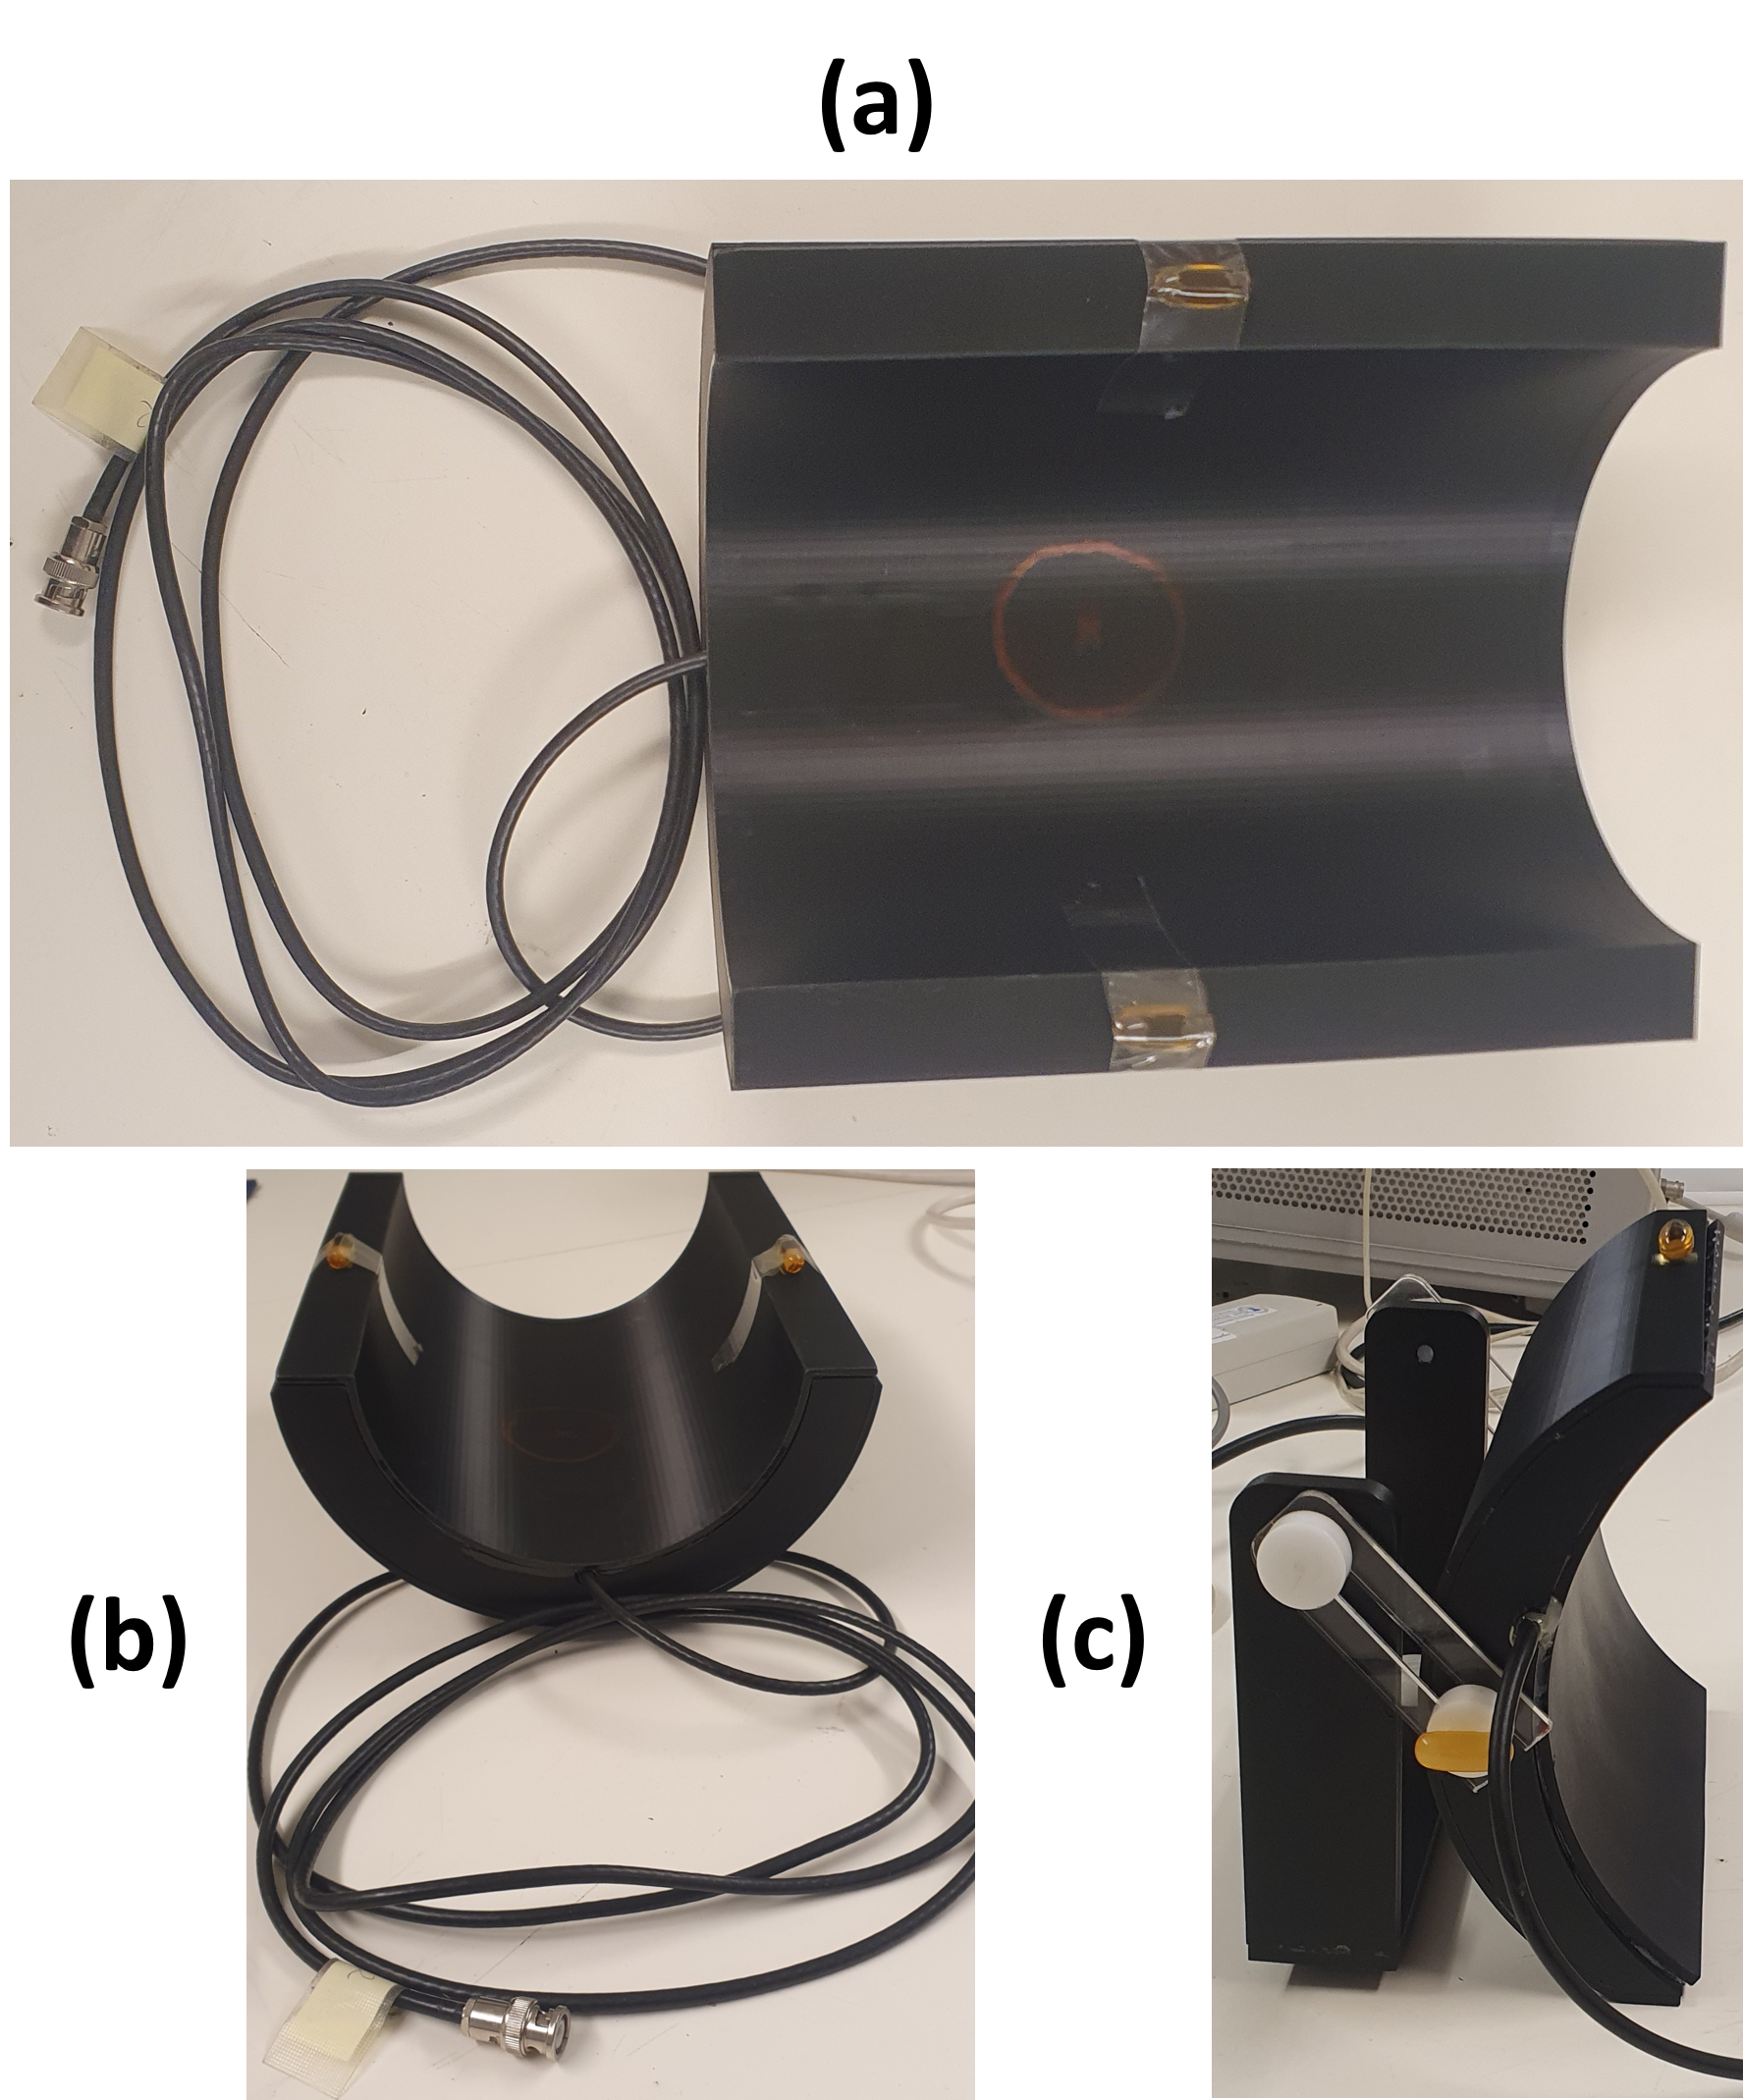
\includegraphics[width=0.9\textwidth]{Figures/Coils/Coil_Pics.png}
    \caption{\textit{Photos of the calf surface coil from two different angles (a \& b) with a photo of the liver surface coil (c), both tuned to the $^2$H Larmor frequency at 3T. The yellow tablets that can be seen in all the photos are vitamin tablets (also known as fiducial markers) used to identify where the coil is in an image.}}
    \label{fig:coils:Pics}
\end{figure}

\subsection{Saddle}

\begin{figure}
    \centering
    \includegraphics[width=1\textwidth]{Figures/Coils/Planar_Saddle.png}
    \caption{\textit{2D circuit diagram of the saddle coil used for scanning of the calf.}}
    \label{fig:coils:2D_Saddle}
\end{figure}

Volumetric coils such as saddle coils have more homogeneous B$_1$ fields than surface coils and are able to cover a larger volume. A saddle coil derives its name from the fact that the coil elements it uses have a similar appearance to a horse's saddle. Two square loops surround a circular tube with an angular separation of 120$^\circ$ of the wires in each saddle. The saddle coil has optimum geometry that has been previously been found which includes the length/diameter between 1 and 2, and an angular width for each coil of $\sim$120$^\circ$ \cite{Ginsberg1970OptimumField,Salmon2006OptimizationImaging}.

\begin{figure}
    \centering
    \includegraphics[width=0.8\textwidth]{Figures/Coils/3D_Saddle.png}
    \caption{\textit{3D circuit diagram of the saddle coil used for scanning of the calf.}}
    \label{fig:coils:3D_Saddle}
\end{figure}

The coil built for scanning in Chapter \ref{Chap:Quad} is made from copper tape and has an angular width of 120$^\circ$ a length of 16.8 cm and a diameter of 14.8 cm. Where the copper tape that links the two squares intersects/crosses over, an insulated wire is used to avoid a capacitor being created. Also, the wires here run close side by side so that the fields from the opposing currents will cancel. Diagrams of the circuit for the coil are shown in Figs. \ref{fig:coils:2D_Saddle} and \ref{fig:coils:3D_Saddle} with pictures in Fig. \ref{fig:coils:Saddle_pic}. The tuning capacitance is 47.3 pF, the total matching capacitance 8.8 pF.

\begin{figure}
    \centering
    \includegraphics[width=1\textwidth]{Figures/Coils/Saddle_Coil.jpg}
    \caption{\textit{Photo of the saddle coil used to obtain $^2$H data from the calf.}}
    \label{fig:coils:Saddle_pic}
\end{figure}

\subsection{Helmholtz coil}

\begin{figure}
    \centering
    \includegraphics[width=0.8\textwidth]{Figures/Coils/Planar_Helmholtz.png}
    \caption{\textit{2D circuit diagram of the Helmholtz coil used for scanning of the arm.}}
    \label{fig:coils:2D_Helmholtz}
\end{figure}

A Helmholtz coil is similar to to a surface coil in its circuitry. Except a second surface coil is connected to it by two crossing insulated wires, where the current in each flows in opposite directions so that the field flows in the centre of the setup. This creates a homogeneous B$_1$ in between the coils. The Helmholtz coil arrangement was chosen for the scanning the forearm described in Chapter \ref{Chap:Quad} and needs to be easily movable and a saddle coil would roll/move to much and would be difficult to rotate in the magnet bore.

\begin{figure}
    \centering
    \includegraphics[width=1\textwidth]{Figures/Coils/3D_Helmholtz.png}
    \caption{\textit{3D circuit diagram of the Helmholtz coil used for scanning of the arm with housing (a) and without (b).}}
    \label{fig:coils:3D_Helmholtz}
\end{figure}

The coil setup comprises involves two octagonal loops that are $\sim$14 cm in diameter separated by a 12 cm gap with a tube in the centre to keep the arm still in the same position, away from the circuit elements. The tuning capacitance is 73.3 pF and the total matching capacitance is 8.8 pF.

\begin{figure}
    \centering
    \includegraphics[width=0.8\textwidth]{Figures/Coils/HelmHoltz_Coil.jpg}
    \caption{\textit{Photo of the HelmHoltz coil used to obtain $^2$H data from the arm.}}
    \label{fig:coils:HelmHoltz_pic}
\end{figure}